\paragraph{Flaw 1}

Flaw 1 is a side-wall crack angled at 35$^{\circ}$ with respect to the normal. It has a length of 30mm, is 6mm tall and the processed images of this flaw can be seen in Figure \ref{fig:AMEC_flaw1}. The reflection from the flaw is strong and the defect can be seen even in the unfiltered TFM image. As expected, the filtered TFM image reduces a significant portion of the noise and allows the defect to be seen more clearly. The SASACI process reduces this noise (measured by taking the mean amplitude in the highlighted area - this area is consistent throughout the following results) by a further 5dB, though the defect is already visible in the previous image and accurate sizing is possible. 

\vspace{20mm}

\begin{figure}[h!]
\centering
		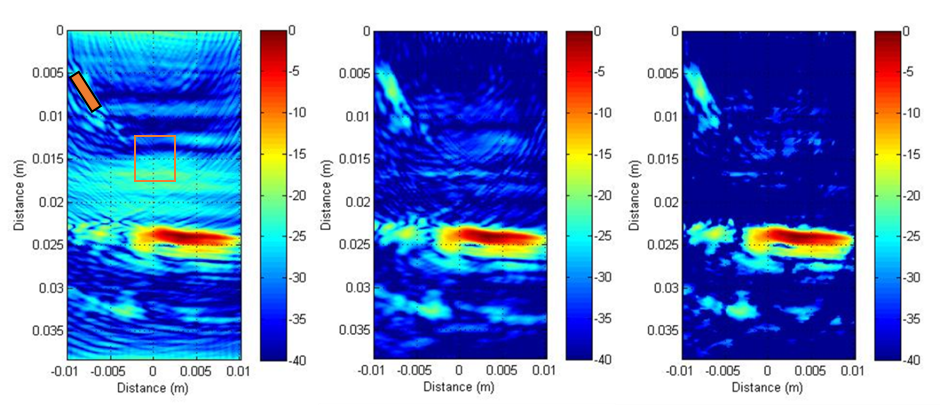
\includegraphics[width=\textwidth]{AMEC5_11.png}
		\caption{TFM, Filtered TFM and SASACI images of Flaw 1 within the stainless steel weld. The side wall crack can be seen clearly at the top left of all three images.}
		\label{fig:AMEC_flaw1}
\end{figure}

\clearpage

\paragraph{Flaw 2}

Flaw 2 is a lack of side wall fusion. It is angled at 40$^{\circ}$ with respect to the normal and has a length and height of 30mm and 6mm respectively. The image results of this flaw are shown in Figure \ref{fig:AMEC_flaw2}. It can be immediately observed from the first of the three images that this section of the weld has much less grain noise compared to the section in which Flaw 1 is located. The background noise level is significantly lower and the defect can be clearly seen. The filtered TFM reduces some of the noise surrounding the backwall and SASACI is able to further reduce some of the noise surrounding the defect.

\vspace{20mm}

\begin{figure}[h!]
\centering
		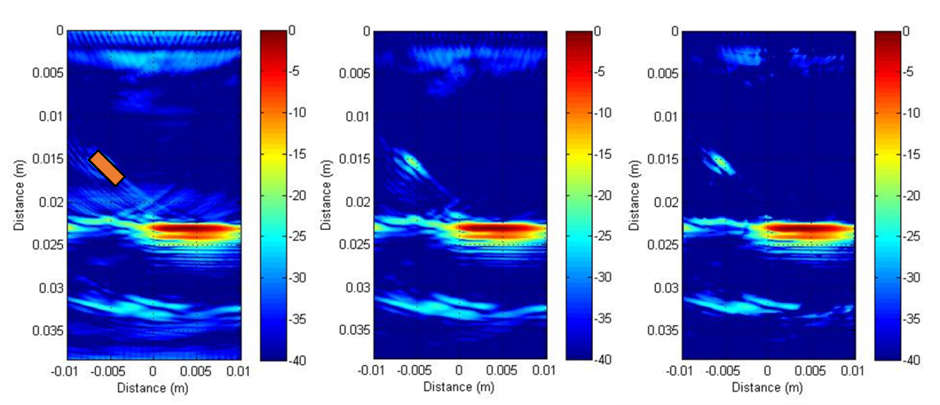
\includegraphics[width=\textwidth]{AMEC6_1.png}
		\caption{TFM, Filtered TFM and SASACI images of Flaw 2 within the stainless steel weld. This defect is a lack of side wall fusion and can be seen approximately 6mm above the back wall on the left hand side of each of the three images.}
		\label{fig:AMEC_flaw2}
\end{figure}

\clearpage

\paragraph{Flaw 3}

Flaw 3 is a vertical centreline crack within the weld. It is 45mm long and 6mm tall. It starts at the bottom of the sample and protrudes upwards. Figure \ref{fig:AMEC_flaw3} shows images of the region in which the flaw is located. No useful information can be observed in the unfiltered TFM image. There is a significant amount of noise surrounding the back wall which hinders analysis of the image. The filtered TFM image reduces noise but it is still not clear where the defect is located. The SASACI image shows further reduced noise, to a point where the top of the defect can be observed. It should be stated that the experimental setup is not optimal for detecting Flaws 3, 4 and 5. To detect vertical flaws, inspection should take place with an angled beam which allows for more energy to be reflected from the defect. A wedge would allow for this.

%\vspace{20mm}

\begin{figure}[h!]
\centering
		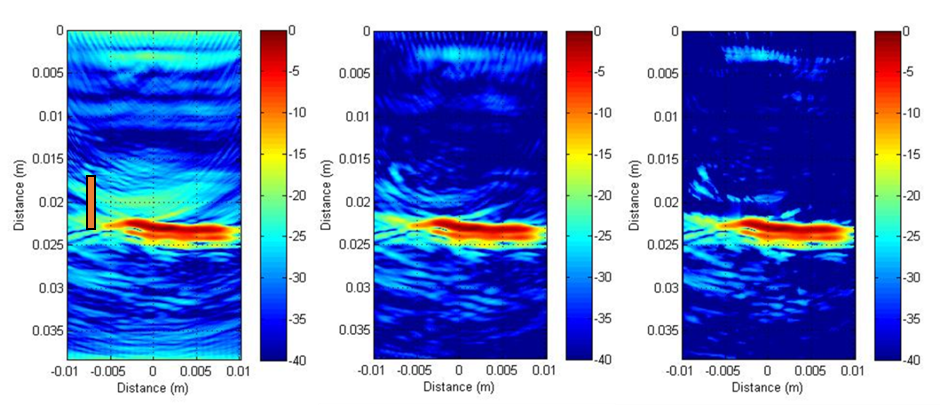
\includegraphics[width=\textwidth]{AMEC7_1.png}
		\caption{TFM, Filtered TFM and SASACI images of Flaw 3 within the stainless steel weld. The centreline crack is expected to be visible in the left hand side of the images and appear as an artefact just above the back wall reflection. It is more prominent in the SASACI image.}
		\label{fig:AMEC_flaw3}
\end{figure}

\clearpage

\paragraph{Flaw 4}

Flaw 4 is also a vertical centreline crack. It is smaller than Flaw 3, being 40mm long and only 5mm tall. This flaw is starts at the top of the sample and protrudes downwards towards the centre of the weld. This flaw cannot be seen in any of the three images shown in Figure \ref{fig:AMEC_flaw4}.

\vspace{20mm}

\begin{figure}[h!]
\centering
		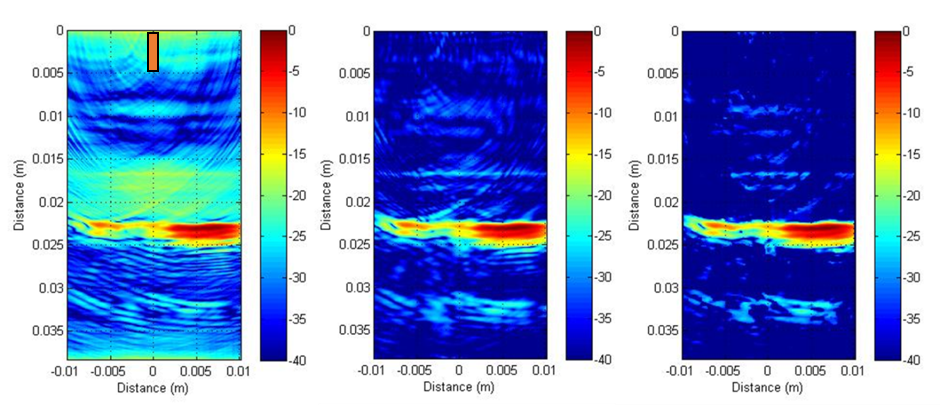
\includegraphics[width=\textwidth]{AMEC8_1.png}
		\caption{TFM, Filtered TFM and SASACI images of Flaw 4 within the stainless steel weld. Flaw 4 is a centreline crack propagating from the top of the weld. Although this defect is not visible in any of the three images, the effects of the crack can be seen as second and third reflections are visible at depths of 8mm and 16mm.}
		\label{fig:AMEC_flaw4}
\end{figure}

\clearpage

\paragraph{Flaw 5}

Flaw 5 is a vertical centreline crack in the centre of the weld. It is larger than the previous flaws and is 50mm in length and 14mm in height. The top of the crack can be seen in the unfiltered TFM image in Figure \ref{fig:AMEC_flaw5}, however the bottom cannot be seen due to the noise around the back wall. The filtered image reduces noise, allowing the top of the crack to be seen clearly. In this case, the bottom of the crack still cannot clearly be seen due to noise. The SASACI image reduces this noise further to a point where the location of the bottom of the crack can be estimated to allow sizing.

\vspace{20mm}

\begin{figure}[h!]
\centering
		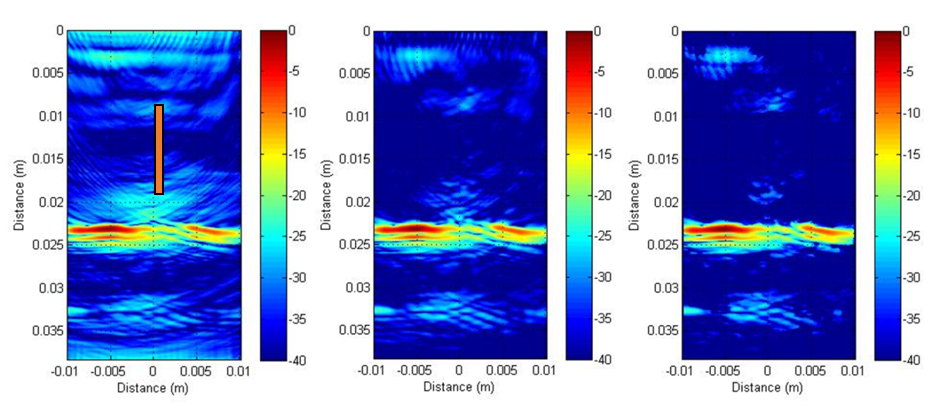
\includegraphics[width=\textwidth]{AMEC9_1.png}
		\caption{TFM, Filtered TFM and SASACI images of Flaw 5 within the stainless steel weld. Flaw 5 is a centreline crack that starts just below the surface and ends just above the back wall of the specimen. The top of the crack can be seen at a depth of 8mm and the bottom is visible at a depth of 20mm. These reflections are most clear in the SASACI image.}
		\label{fig:AMEC_flaw5}
\end{figure}

\clearpage

\paragraph{Flaw 6}

Flaw 6 is a lack of side wall fusion and is at an angle of 35$^{\circ}$ with respect to the normal. The crack is sized 50mm in length and 4mm tall. Figure \ref{fig:AMEC_flaw6} shows the three images related to this defect. The unfiltered TFM image is very noisy due to the grain structure within the weld. The bandpass filtering reduces noise to the point where the defect can be seen above the noise and SASACI further reduces this noise by around 10dB. 

\vspace{20mm}

\begin{figure}[h!]
\centering
		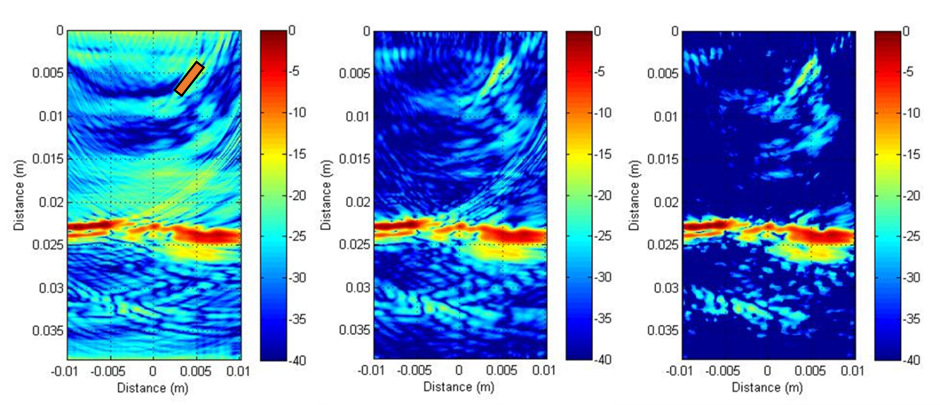
\includegraphics[width=\textwidth]{AMEC10_1.png}
		\caption{TFM, Filtered TFM and SASACI images of Flaw 6 within the stainless steel weld. This defect is a lack of side wall fusion and can be seen at the top-right of both the filtered and SASACI images. The defect is clearest in the SASACI image due to the reduced noise in the image.}
		\label{fig:AMEC_flaw6}
\end{figure}

\clearpage

\paragraph{Flaw 7}

Flaw 7 is a transverse crack at the top of the sample and is 40mm long and 4mm in height. This defect cannot be seen in any of the three images represented in Figure \ref{fig:AMEC_flaw7}. The filtered TFM and SASACI images show clear horizontal artefacts that are also present in Flaw 4. While the defects near the top of the sample cannot be seen in any of the images, it is possible that the flaws are contributing to these artefacts. The orientation of this defect is such that it is expected to be found. There is currently no explanation for the fact that the defect cannot be seen in any of the images.

\vspace{20mm}

\begin{figure}[h!]
\centering
		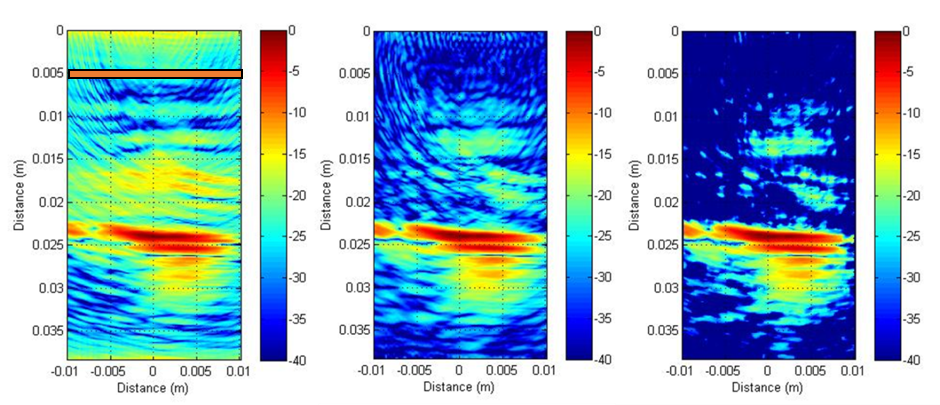
\includegraphics[width=\textwidth]{AMEC11_1.png}
		\caption{TFM, Filtered TFM and SASACI images of Flaw 7 within the stainless steel weld. Flaw 7 is a transverse crack propagating 4mm into the material from the top surface. It is not visible in any of the three images, though the effects can be seen as a large artefact is visible at a depth of around 13mm in both the filtered and SASACI images.}
		\label{fig:AMEC_flaw7}
\end{figure}

